\documentclass[8 pt, twocolumn]{article}

\usepackage[utf8x]{inputenc}
\usepackage{dsfont}
\usepackage{amsthm}
\usepackage{amsfonts}
\usepackage{amssymb}
\usepackage{tensor}
\usepackage{mathtools}
\usepackage[T1]{fontenc}
%\usepackage[spanish]{babel}
\usepackage[cm]{fullpage}
\usepackage{graphicx}
\usepackage{float}
\usepackage{bm}
\usepackage{setspace}
\usepackage{enumitem}
\usepackage{mdwlist}
\usepackage{parskip}
\usepackage{listings}
\usepackage{color}
%\usepackage{epstopdf}
\usepackage{tikz,datatool}
\usepackage{hyperref}

\newcommand{\HRule}{\rule{\linewidth}{0.5mm}}

\AtBeginDocument{
  \let\myThePage\thepage
  \renewcommand{\thepage}{\oldstylenums{\myThePage}}
}

\newcommand{\gra}{$^\text{o}$}
\newcommand{\dif}{\text{d}}
\newcommand{\avg}[1]{\left\langle #1 \right\rangle}
\newcommand{\ket}[1]{\left| #1 \right\rangle}
\newcommand{\bra}[1]{\left\langle #1 \right|}
\newcommand{\bket}[2]{\left\langle #1 \middle| #2 \right\rangle}
\newcommand{\der}[2]{\frac{\text{d} #1}{\text{d} #2}}
\newcommand{\prt}[2]{\frac{\partial #1}{\partial #2}}
\newcommand{\dert}[3]{\frac{\text{d}^#3 #1}{\text{d} #2^#3}}
\newcommand{\prtt}[3]{\frac{\partial^#3 #1}{\partial #2^#3}}
\newcommand{\dl}{\mathcal{L}}
\newcommand{\dha}{\mathcal{H}}
\newcommand{\vol}{\text{vol}}
\renewcommand{\vec}[1]{\pmb{#1}}

\newenvironment{algo}[1]
{  \begin{center}
   \mbox{
       \begin{minipage}{\textwidth}
           \begin{tabbing}
           \settabs
            #1
           \end{tabbing}
        \end{minipage}
    }
    \end{center}
}{}
\newcommand{\settabs}{mmm\=mmm\=mmm\=mmm\=mmm\=mmm\=\kill}

\DeclarePairedDelimiter\ceil{\lceil}{\rceil}
\DeclarePairedDelimiter\floor{\lfloor}{\rfloor}

\definecolor{mygray}{rgb}{0.4,0.4,0.4}
\definecolor{mygreen}{rgb}{0,0.5,0.25}
\definecolor{myorange}{rgb}{1.0,0.4,0}

\definecolor{clock0}{cmyk}{1,0,0,0}
\definecolor{clock1}{cmyk}{1,1,0,0}
\definecolor{clock2}{cmyk}{0,1,0,0}
\definecolor{clock3}{cmyk}{0,1,1,0}
\definecolor{clock4}{cmyk}{1,0,1,0}
\definecolor{clock5}{cmyk}{1,1,1,0}
\definecolor{clock6}{cmyk}{0,0,1,0}
\definecolor{clock7}{cmyk}{0,0,0,0.1}

\begin{document}

\lstset{
language=C++,
basicstyle=\ttfamily\color{black},
commentstyle=\color{mygray}\ttfamily,
frame=single,
numbers=left,
numbersep=5pt,
numberstyle=\tiny\color{mygray}\ttfamily,
keywordstyle=\color{mygreen}\ttfamily,
showspaces=false,
showstringspaces=false,
stringstyle=\color{myorange}\ttfamily,
tabsize=2,
emph={double,uint8_t,uint16_t,uint32_t,uint64_t,int8_t,int16_t,int32_t,int64_t},
emphstyle={\color{blue}\ttfamily}
}

\begin{minipage}[b]{\linewidth}
  \centering
  \Large \textsc{Numerical analysis of the phase transition in the Ising Model}\\
  ~\\
  \large \textsc{Francisco García Flórez}
\end{minipage}

\section{Introduction}

% Phase transition, critical temperature, critical exponents, universality class.

\section{General considerations}

% Hamiltonian, Size of the system, metropolis and wolff, thermalization, 2d and 3d

In this project we are going to consider the following Hamiltonian for the system

\begin{equation} H = - J \sum_{\avg{ij}} s_i s_j - B \sum_i s_i \text{ ,} \end{equation}

where $J$ and $B$ are positive constants, referencing respectively the alignment energy and a possible external magnetic field, which we will consider zero for the first part of this study. Since this is a numerical simulation of the Ising model, there are several core remarks that we will explicitly state in the following.

\subsection{System size, boundary conditions and dimensionality}

Firstly, we will consider systems with different numbers of lattice points, defined as $N=L^d$, that we will use to increase the precision of some measurements and avoid size-specific effects. In relation to this remark, since we cannot simulate an infinite system we are imposing helical boundary conditions, defined as

\begin{equation} s_i = s_{\mod(i\pm L^n, N)} ~~ \forall n \in [0,d) \text{ ,} \end{equation}

where $d$ is the space dimension of the system. We are going to be considering both 2D and 3D systems only, but we will keep our expressions as dimension-independent as possible.

\subsection{Monte-Carlo algorithms}

This is a Monte-Carlo simulation of the Ising model, meaning we will compute several quantities like Energy or Magnetization using different configurations of the system. To find these configurations we will follow two different algorithms: Metropolis and Wolff's. We are not going to go into the details of how and why they work, just the basics:

\begin{itemize}
  \item \textbf{Metropolis algorithm with single spin-flip dynamics.} As the name suggests, we will be performing single lattice point spin flips, $N$ of them per simulation step. Because it's a Metropolis algorithm the acceptance ratio is given by

  \begin{equation} A(\mu \rightarrow \nu) = \left\{ \begin{matrix} e^{-\beta(E_\nu-E_\mu)} & \text{ if } E_\nu - E_\mu > 0 \\
  1 & \text{otherwise} \end{matrix} \right. \text{ .} \end{equation}

  Since each lattice point will be picked, on average, the same amount of times we will use simulation steps per lattice site as the unit of measure for time in every simulation generated with this algorithm.

  \item \textbf{Wolff's algorithm.} In this case we are not going to flip only one spin, but instead we will look for clusters of parallel spins and flip all of them with some probability. Using this algorithm near the critical point increases significantly the speed of the simulation. The probability of adding one extra spin to the cluster can be chosen to be

  \begin{equation} P_{\text{add}} = 1 - e^{-2\beta J} \text{ .} \end{equation}

  In this case we cannot use simulation steps per lattice point as a constant unit, so instead we will  cluster flips as time for this algorithm. In the implementation we choose one cluster flip per simulation step, so in the following we will simply call $t$ ``Simulation steps''.
\end{itemize}

\subsection{Autocorrelation functions and Correlation time $\tau$}

Finally, for all these simulations to work we need to compute averages of quantities once the system has reached equilibrium, process also known as \emph{thermalization}. There are several methods to check whether or not the system has equilibrated, but the simplest one is looking at the Magnetization and Energy as a function of simulation steps (per lattice point).

\begin{figure}[H]
  \begin{center}
    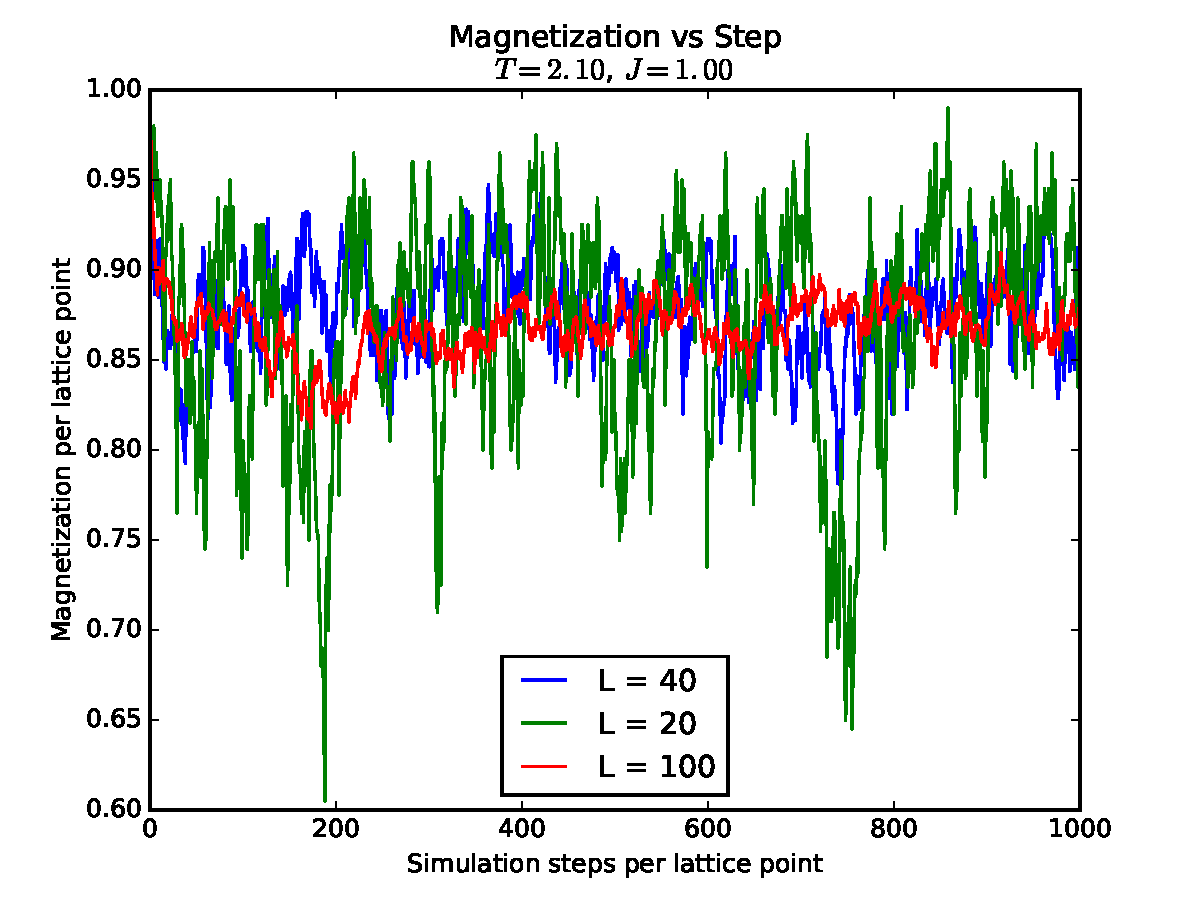
\includegraphics[width=0.45\textwidth]{{../graphs/MvsN}.pdf}
  \end{center}
  \caption{Plot of the magnetization per lattice point as a function of simulation steps per lattice point (sslp), using Metropolis algorithm.}
\end{figure}

In this plot we can easily see a thermalization time of around 100 sslp, however, as we could expect it depends heavily on $T$. In this simulation we are starting from a system with uniform spins, equivalent to a system at exactly $T=0$, and thus the system equilibrates quicker at $T=2.1$ (as shown in the plot) than at $T=10$, after the phase transition. Later on we will take a second look at this.

Next, we can do the same with Wolff's algorithm to find:

\begin{figure}[H]
  \begin{center}
    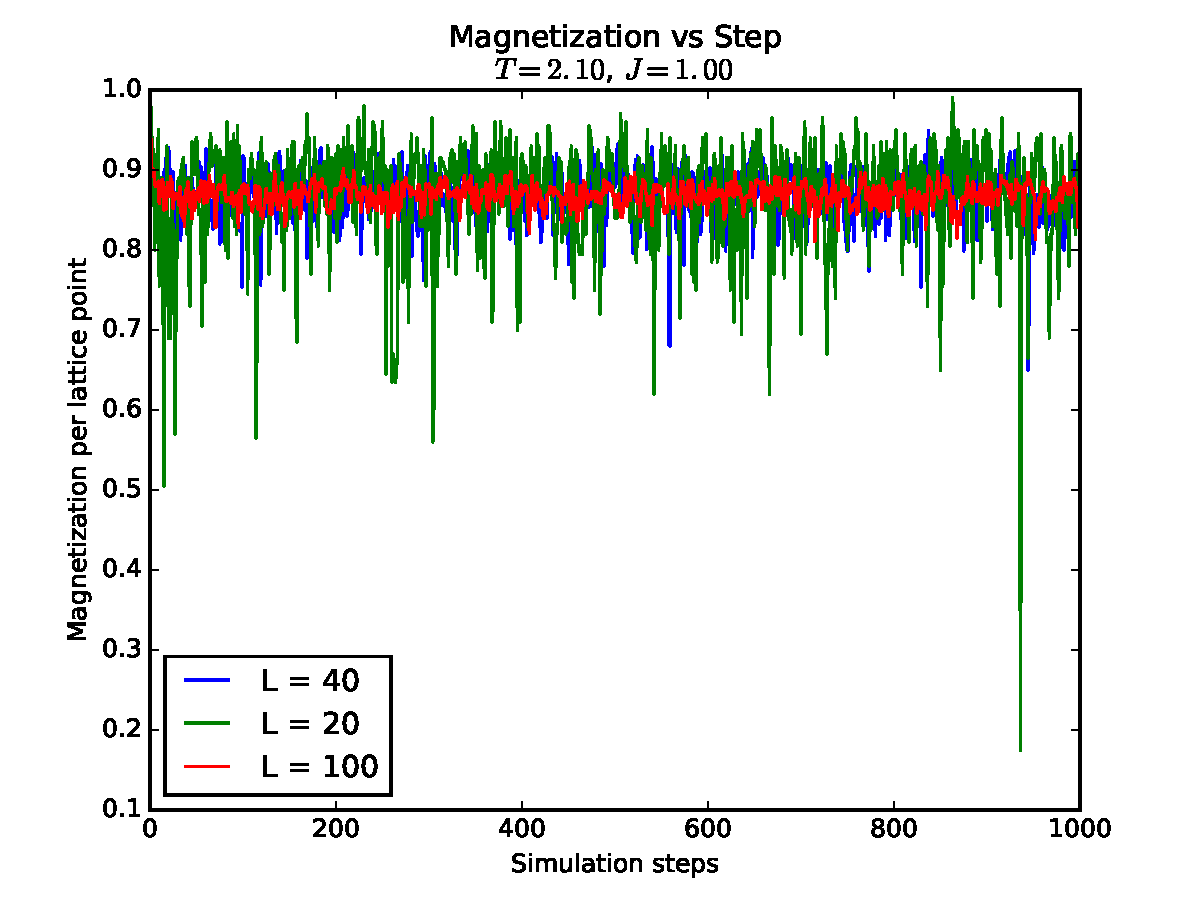
\includegraphics[width=0.45\textwidth]{{../graphs/MvsN-wolff}.pdf}
  \end{center}
  \caption{Plot of the magnetization per lattice point as a function of simulation steps, using Wolff's algorithm.}
\end{figure}

Of course, this algorithm provides significantly lower correlation times, as we will see later it's around 10 to 20 simulation steps. Plotting the energy as a function of steps would gives a similar result, so we can omit the explicit plot. There is a better way to compute how much time should we wait, and it involves computing what is called autocorrelation function. We can compute this both using the energy or the magnetization, using the following expression

\begin{equation} \label{eq:autocorrelation} \begin{matrix} \xi_M(t) =  & \frac{1}{t_{\text{max}} - t} \sum_{t'=0}^{t_{\text{max}}-t} M(t')M(t'+t) \\
             & - \frac{1}{t_{\text{max}} - t} \sum_{t'=0}^{t_{\text{max}}-t} M(t') \\
             & \times \frac{1}{t_{\text{max}} - t} \sum_{t'=0}^{t_{\text{max}}-t} M(t'+t) \end{matrix} \text{ .} \end{equation}

And equivalently for the energy. From $\xi(t)$ we can compute the correlation time $\tau$ as

\begin{equation} \tau = \frac{1}{\xi(0)} \int_0^\infty \dif t \xi(t) \text{ ,} ~~~~ \xi(0) = \avg{M^2} - \avg{|M|}^2 \text{ ,}  \end{equation}

where we could change $M(t)$ by $E(t)$ and do the same with the energy. Firstly, using equation (\ref{eq:autocorrelation}) we find the following results, using the Metropolis algorithm, for magnetization:

\begin{figure}[H]
  \begin{center}
    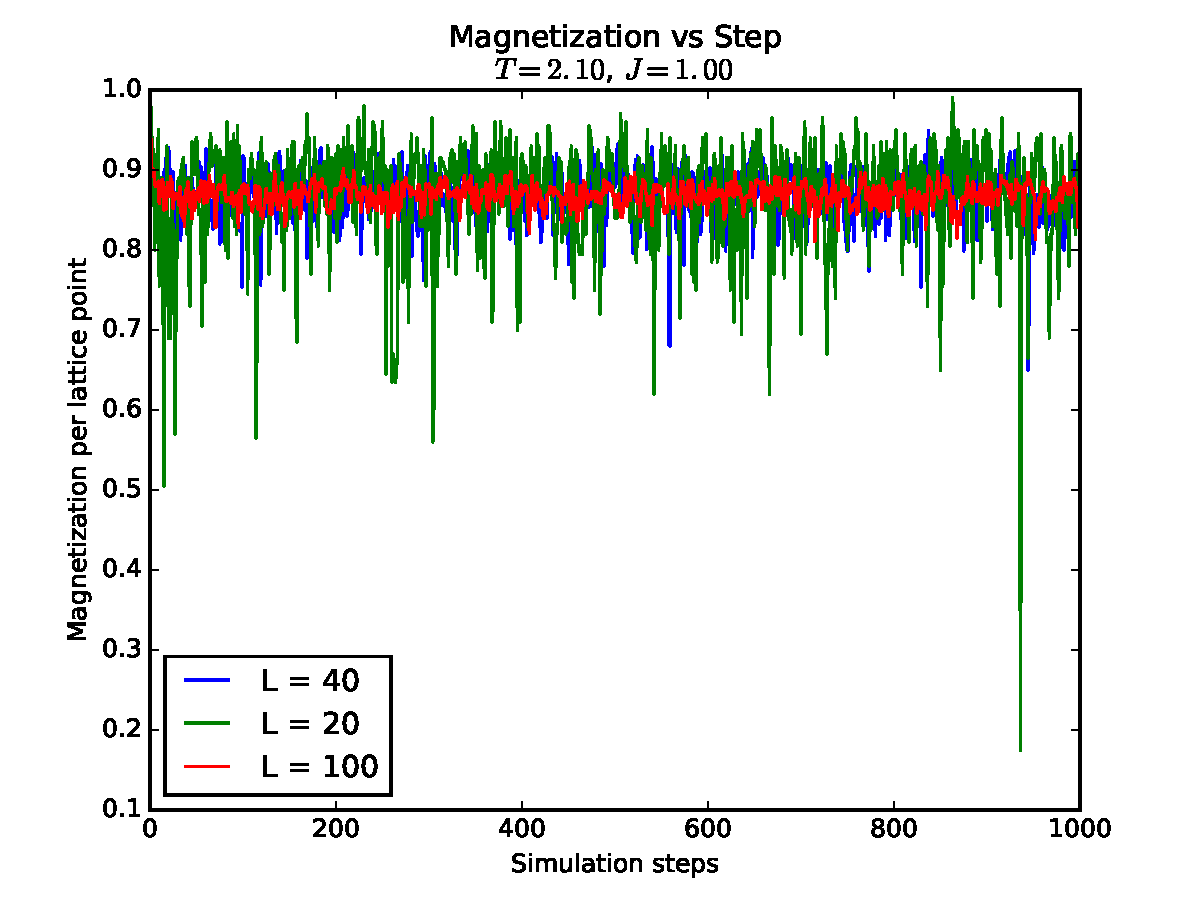
\includegraphics[width=0.45\textwidth]{{../graphs/MvsN-wolff}.pdf}
  \end{center}
  \caption{Plot of the autocorrelation function $\xi(t)$ using magnetization.}
\end{figure}

And energy:

\begin{figure}[H]
  \begin{center}
    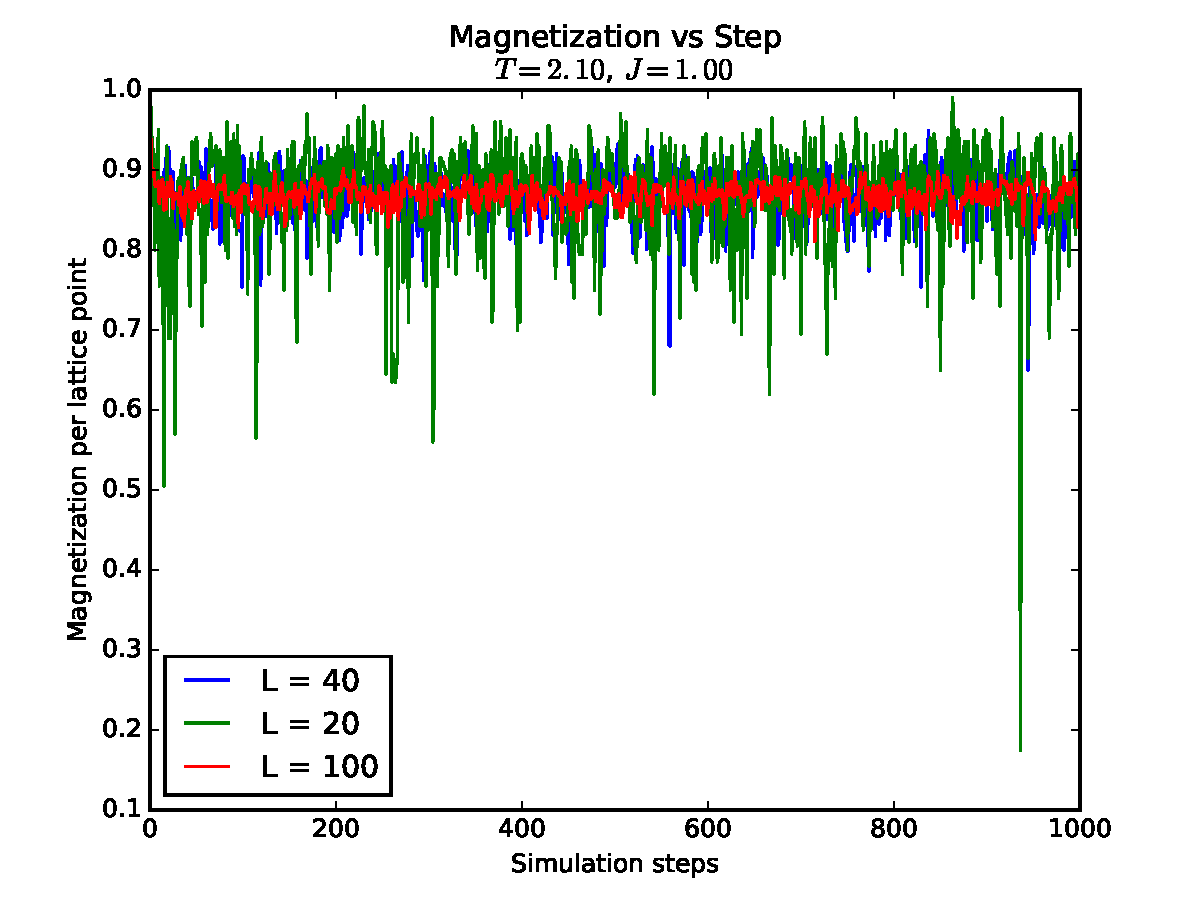
\includegraphics[width=0.45\textwidth]{{../graphs/MvsN-wolff}.pdf}
  \end{center}
  \caption{Plot of the autocorrelation function $\xi(t)$ using energy.}
\end{figure}



\section{Phase transition}

\subsection{Energy $E(T)$ and Magnetization $|M(T)|$}

\subsection{Specific Heat $c_s(T)$ and Magnetic Susceptibility $\chi(T)$}

\subsection{Critical exponents}


\end{document}
